\documentclass[dvipdfmx,11pt,notheorems]{beamer}
%%%% 和文用 %%%%%
\usepackage{bxdpx-beamer}
\usepackage{pxjahyper}
\usepackage{minijs}%和文用
\renewcommand{\kanjifamilydefault}{\gtdefault}%和文用

%%%% スライドの見た目 %%%%%
\usetheme{Madrid}
\usefonttheme{professionalfonts}
\setbeamertemplate{frametitle}[default][center]
\setbeamertemplate{navigation symbols}{}
\setbeamercovered{transparent}%好みに応じてどうぞ)
\setbeamertemplate{blocks}[rounded]
\useinnertheme{circles}
%\setbeamertemplate{footline}[page number]
%\setbeamerfont{footline}{size=\normalsize,series=\bfseries}
%\setbeamercolor{footline}{fg=black,bg=black}
%%%%

%%%% 定義環境 %%%%%
\usepackage{amsmath,amssymb}
\usepackage{amsthm}
\theoremstyle{definition}
\newtheorem{theorem}{定理}
\newtheorem{definition}{定義}
\newtheorem{proposition}{命題}
\newtheorem{lemma}{補題}
\newtheorem{corollary}{系}
\newtheorem{conjecture}{予想}
\newtheorem*{remark}{Remark}
\renewcommand{\proofname}{}
%%%%%%%%%

%%%%% フォント基本設定 %%%%%
\usepackage[T1]{fontenc}%8bit フォント
\usepackage{textcomp}%欧文フォントの追加
\usepackage[utf8]{inputenc}%文字コードをUTF-8
\usepackage[deluxe]{otf}%otfパッケージ
\usepackage{lxfonts}%数式・英文ローマン体を Lxfont にする
\usepackage{bm}%数式太字
%%%%%%%%%%

%%%%% PythonTeX %%%%%
\usepackage[makestderr]{pythontex}
\restartpythontexsession{\thesection}
 
\title[All about cmath module]{君はcmathを知っているか}
\author[Hayao]{Hayao Suzuki}
\institute[Shizuoka 2020]{PyCon mini Shizuoka 2020}
\date{February 29, 2020}

\begin{document}

\begin{frame}[plain]\frametitle{}
\titlepage %表紙
\end{frame}

\begin{frame}\frametitle{Contents}
\tableofcontents %目次
\end{frame}

\section{自己紹介}

\begin{frame}\frametitle{自己紹介}

\begin{block}{お前誰よ}
\begin{description}
\item[名前] Hayao Suzuki(鈴木 駿)
\item[Twitter] \href{https://twitter.com/CardinalXaro}{@CardinalXaro}
\item[ブログ] \url{https://xaro.hatenablog.jp/}
\item[専門] 数学 (組合せ論・グラフ理論)
\item[学位] 修士(工学)、\href{https://www.uec.ac.jp/}{電気通信大学}
\item[仕事] \href{https://iridge.jp/}{株式会社アイリッジ}
\begin{itemize}
\item スマートフォンアプリのバックエンドサーバーの開発
\item 酢豆腐スペシャリスト
\end{itemize}
\end{description}
\end{block}

\end{frame}

\begin{frame}\frametitle{自己紹介}

\begin{block}{技術書の査読}
\begin{itemize}
\item 『Effective Python』(オライリージャパン)
\item 『エレガントなSciPy』(オライリージャパン)
\item 『データサイエンス設計マニュアル』(オライリージャパン)など
\item \url{https://xaro.hatenablog.jp/}に一覧あります。
\end{itemize}
\end{block}

\begin{block}{いろんな発表}
\begin{itemize}
\item 「SymPyによる数式処理」(PyCon JP 2018)
\item 「Pythonで楽しむ初等整数論」(PyCon mini Hiroshima 2019)など
\item \url{https://xaro.hatenablog.jp/}に一覧あります。
\end{itemize}
\end{block}

\end{frame}

\section{cmathとは何者か}

\begin{frame}\frametitle{今日の発表}

\begin{exampleblock}{\texttt{cmath}とは何者か}
\begin{enumerate}
\item C言語で実装された高速な\texttt{math}ライブラリ
\item キュウリ(Cucumber)の画像識別のための数学ライブラリ
\item 複素数(Complex Number)の計算ライブラリ
\end{enumerate}

\end{exampleblock}

\end{frame}

\begin{frame}\frametitle{今日の発表}

\begin{block}{バッテリー同梱哲学(\href{https://www.python.org/dev/peps/pep-0206/}{PEP 206}より)}
Pythonディストリビューション自身が、別途ダウンロードすることなく
すぐに利用できる豊富で汎用性の高い標準ライブラリを持つこと。
\end{block}

\begin{exampleblock}{Pythonチュートリアルで紹介されている例}
\begin{itemize}
\item \structure{\texttt{xmlrpc.client}} XML-RPC クライアント
\item \structure{\texttt{xmlrpc.server}} XML-RPCサーバー
\item \structure{\texttt{email}} 電子メールとMIME 処理のためのパッケージ
\item \structure{\texttt{json}} JSONエンコーダおよびデコーダ
\item \structure{\texttt{sqlite3}} SQLiteデータベースに対するDB-API 2.0インタフェース
\end{itemize}
\end{exampleblock}

\end{frame}

\begin{frame}\frametitle{今日の発表}

\begin{block}{\texttt{cmath}モジュール}
\begin{itemize}
\item 複素数のための数学関数
\item 9V電池やらニカド電池のような存在に今、スポットを当てる。
\end{itemize}
\end{block}

\begin{block}{今回使うもの}
\begin{itemize}
\item Python 3.7.x(Python 3.8.xでも楽しめます!)
\item Matplotlib(グラフ描画ライブラリ)
\end{itemize}
\end{block}

\end{frame}

\begin{frame}\frametitle{今日の発表}

\begin{block}{君は\texttt{cmath}を知っているか}
\begin{itemize}
\item \texttt{cmath}とは何者か
\item 複素数とは何か
\item 複素数の極座標表記
\item 複素指数函数
\item 離散Fourier変換
%\item Mandelbrot集合
\item 1の$n$乗根
\item まとめ
\end{itemize}
\end{block}

\begin{exampleblock}{資料は設計図共有サイトにある!}
資料はすべて
\url{https://github.com/HayaoSuzuki/PyCon-mini-Shizuoka-2020/}
にあります。
\end{exampleblock}

\end{frame}

\section{複素数とは何か}

\begin{frame}\frametitle{複素数とは}

\begin{center}
\Huge{複素数、知ってますか?}
\end{center}

\end{frame}

\begin{frame}[fragile]\frametitle{複素数の定義}

\begin{definition}[複素数]
$i^{2}=-1$であるような基底が$1, i$を持つ
実数体$\mathbf{R}$上の2次元ベクトル空間の元を複素数と呼ぶ。
また、$i$を虚数単位と呼ぶ。
\end{definition}

\begin{exampleblock}{Pythonで複素数を定義する}
\begin{pyconsole}
3 + 5j # Pythonでは虚数単位をjまたはJとする
(0 + 1J)**2 # 虚数単位の自乗は-1となる。
4 + 5j == (5j + 4) # 実部と虚部がそれぞれ等しい
\end{pyconsole}
\end{exampleblock}

\end{frame}

\begin{frame}[fragile]\frametitle{複素数と体}

\begin{block}{体(Field) == 四則演算ができる集合}
複素数は複素数体$\mathbf{C}$をなす。
\end{block}

\begin{exampleblock}{Pythonにおける複素数の四則演算}
\begin{pyconsole}
8 - 5j + -5 + 1j # 加法
(1 + 2j) * (1 - 2J) # 乗法
(97 + 0j) / (4 + 9j) # 除法
\end{pyconsole}
\end{exampleblock}

\end{frame}

\begin{frame}[fragile]\frametitle{複素数と順序}
\begin{block}{複素数体は順序体ではない}
実数のような全順序関係を定義できない!
\end{block}

\begin{exampleblock}{Pythonも複素数体は順序体ではないことを知っている}
\begin{pygments}{python}
>>> -100 - 100j < 65536 + 256j # 右辺が大きそうに思えるが...
\end{pygments}
\begin{pygments}{python}
Traceback (most recent call last):
  File "<stdin>", line 1, in <module>
TypeError: '<' not supported between 
instances of 'complex' and 'complex'
\end{pygments}
\end{exampleblock}
\end{frame}

\begin{frame}[fragile]\frametitle{複素数の共役}

\begin{block}{複素数の共役}
複素数$z=x + iy$に対して$\bar{z}=x -iy$を$z$の共役と呼ぶ。
\end{block}

\begin{exampleblock}{Pythonにおける複素数の共役}
\begin{pyconsole}
z = 5 - 3j
z.conjugate()  # complex型のメソッドとして
\end{pyconsole}
\end{exampleblock}

\begin{alertblock}{共役の説明はどこにある?}
組み込み型や\texttt{cmath}ではなく\texttt{numbers}モジュールで説明されている。
\end{alertblock}

\end{frame}

\section{複素数の極座標表記}

\begin{frame}\frametitle{複素数の極座標表記}

\begin{block}{複素数平面}
複素数$z=x + iy$を2次元実数平面$\mathbf{R}^{2}$上の点$(x, y)$とみなすことができる。これを複素数平面という。
\end{block}

\begin{block}{複素数の極座標形式}
複素数平面上の点$z=x+iy (x, y \in \mathbf{R})$を実部$x$と虚部$y$の組$(x, y)$ではなく原点からの距離$r$と偏角$\theta $の組$(r, \theta )$でも定義できる。
これを複素数の極座標形式という。
\end{block}

\end{frame}

\begin{frame}\frametitle{複素数の極座標表記}

\begin{block}{百聞は一見に然り}
\begin{figure}
  \centering
  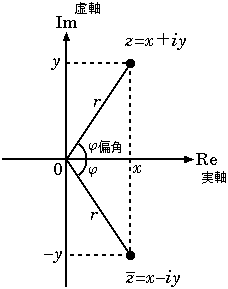
\includegraphics[width=4cm]{complex_plane.png}
  \caption{複素数平面(Wikipediaから引用)}
\end{figure}
\end{block}
\end{frame}

\begin{frame}[fragile]\frametitle{Pythonにおける複素数の極座標表記}
\begin{exampleblock}{Pythonにおける複素数の四則演算}
\begin{pyconsole}
import cmath  # 真打登場
z = 1 + 2j  # 直交座標から極座標に変換する
r, phi = cmath.polar(z)
r, phi  # r = abs(z), phi = cmath.phase(z)
w = cmath.rect(r, phi)  # 極座標から直交座標に変換する
w
cmath.isclose(z, w)  # == ではなくiscloseを使う
\end{pyconsole}
\end{exampleblock}

\end{frame}


\section{複素指数函数}

\begin{frame}\frametitle{指数函数}

\begin{block}{指数函数\texttt{cmath.exp(x)}(公式ドキュメントより)}
$e$を自然対数の底として、$e$の$x$乗を返します。
\end{block}

\begin{alertblock}{自然対数の底の複素数乗って何???}
\begin{itemize}
\item 自然数乗 $\rightarrow$ わかる
\item 整数乗 $\rightarrow$ わかる
\item 有理数乗 $\rightarrow$ まだわかる
\item 実数乗 $\rightarrow$ まだこれなら...
\item 複素数乗 $\rightarrow$ これもうわかんねぇな
\end{itemize}
\end{alertblock}

\end{frame}

\begin{frame}\frametitle{指数函数を巡る冒険}

\begin{block}{極限で定義すればいいんだ!}
\begin{equation*}
e^{z} := \lim_{n \to \infty}\left ( 1 + \frac{z}{n} \right )^{n}.
\end{equation*}
\end{block}

\begin{block}{無限級数で定義すればいいんだ!}
\begin{equation*}
e^{z} := \sum^{\infty}_{n=0}\frac{z^{n}}{n!}.
\end{equation*}
\end{block}

\begin{block}{実函数で定義すればいいんだ!}
\begin{equation*}
e^{z} := e^{x}(\cos{y}+i\sin{y}) 
\end{equation*}
where $z = x + iy$.
\end{block}

\end{frame}

\begin{frame}[fragile]\frametitle{指数函数を巡る冒険}

\begin{exampleblock}{極限値による定義}
\begin{pygments}{python}
def exp_by_limit(z: complex, n: int = 10) -> complex:
    N = 10 ** n
    return pow(1 + z / N, N)
\end{pygments}
\end{exampleblock}

\begin{exampleblock}{無限級数による定義}
\begin{pygments}{python}
def exp_by_series(z: complex, n: int = 30) -> complex:
    return sum(pow(z, i) / factorial(i) for i in range(n))
\end{pygments}
\end{exampleblock}

\begin{exampleblock}{実函数による定義}
\begin{pygments}{python}
def exp_by_real_func(z: complex) -> complex:
    x, y, i = z.real, z.imag, (0 + 1j)
    return math.exp(x) * (math.cos(y) + math.sin(y) * i)
\end{pygments}
\end{exampleblock}

\end{frame}

\begin{frame}[fragile]\frametitle{見せてもらおうか、\texttt{cmath.exp}の威力とやらを}
\begin{exampleblock}{自作の関数でEulerの等式$e^{i\pi} = -1$を計算してみる}
\begin{pygments}{python}
>>> z = cmath.pi * (0 + 1j)
>>> exp_by_limit(z)
(-1.0004936019770099+1.0340526558763341e-07j)
>>> exp_by_series(z)
(-1.0000000000000002+3.461777852236587e-16j)
>>> exp_by_real_func(z)
(-1+1.2246467991473532e-16j)
\end{pygments}
\end{exampleblock}

\begin{exampleblock}{\texttt{cmath.exp}でEulerの等式$e^{i\pi} = -1$を計算してみる}
\begin{pygments}{python}
>>> cmath.exp(z)
(-1+1.2246467991473532e-16j)
\end{pygments}
\end{exampleblock}

\end{frame}

\section{離散Fourier変換}

\begin{frame}[fragile]\frametitle{離散Fourier変換}

\begin{block}{離散Fourier変換}
複素函数$f(x)$の離散Fourier変換$F(t)$は

\begin{equation*}
F(t) = \sum^{N-1}_{n=0}f(n)e^{-i \frac{2\pi n  t }{N}}
\end{equation*}
で与えられる。
\end{block}

\end{frame}

\begin{frame}[fragile]\frametitle{離散Fourier変換}

\begin{block}{例:信号解析}
\begin{figure}
  \centering
  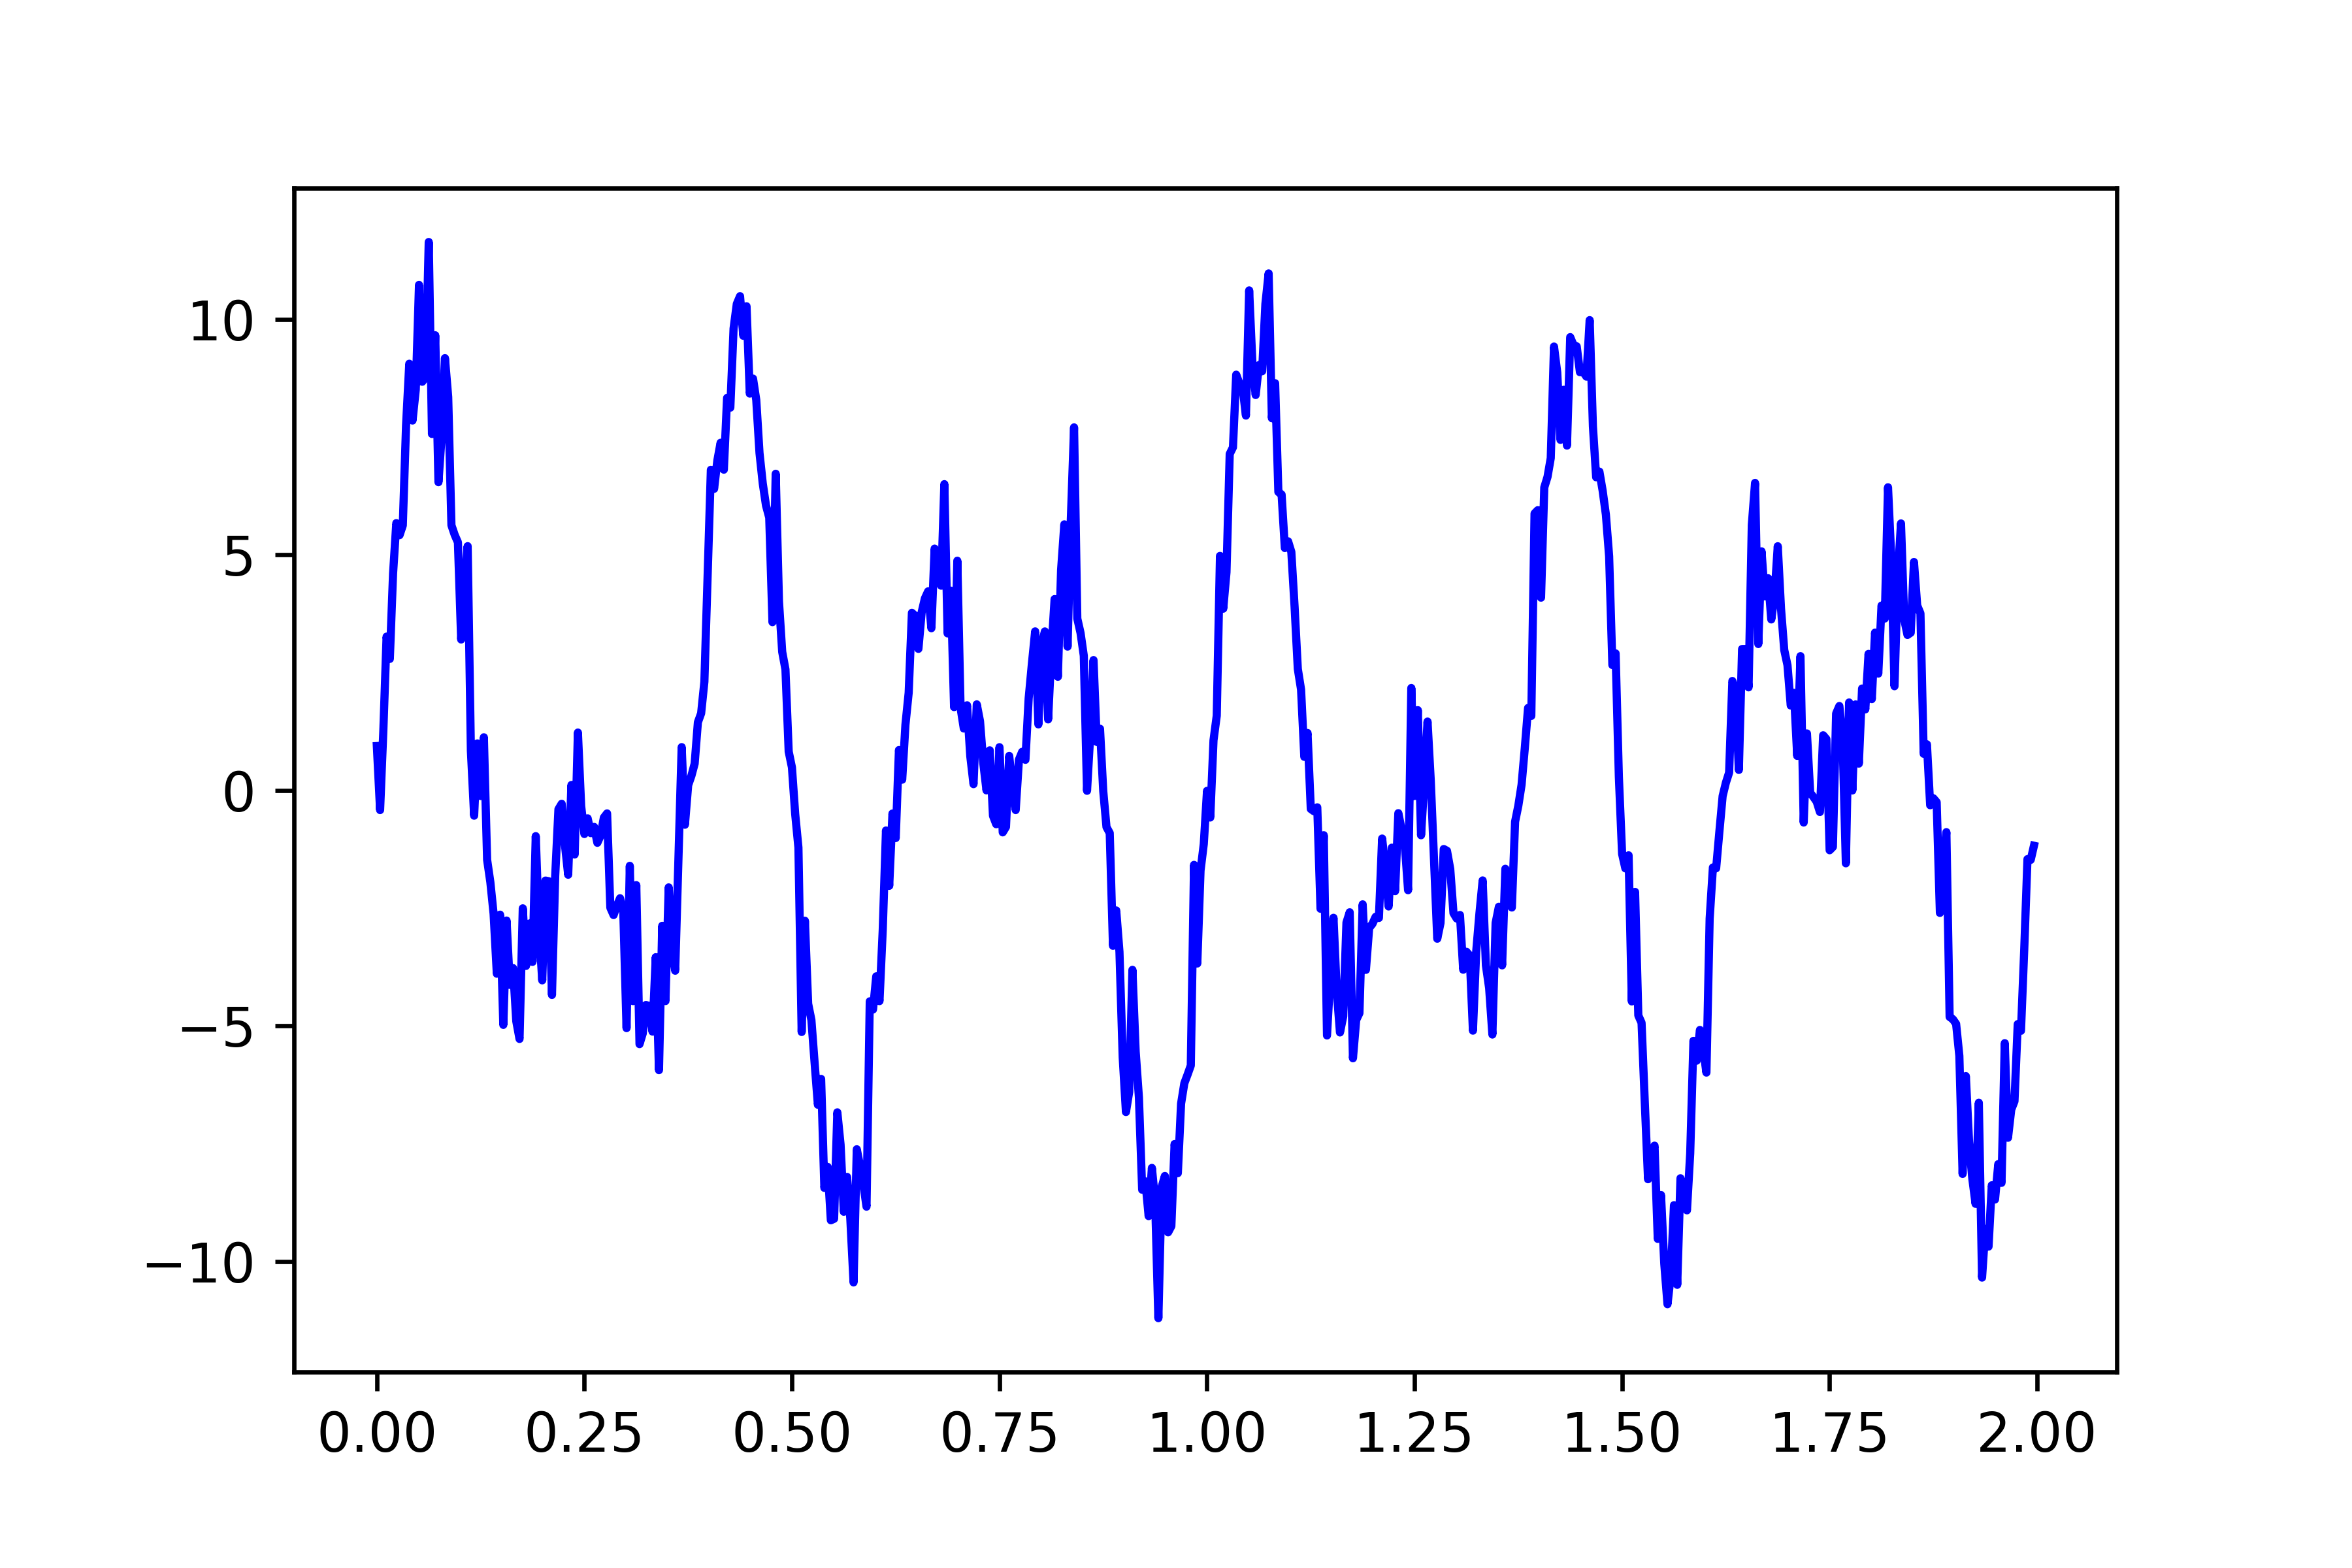
\includegraphics[width=8cm]{sine_curve.png}
  \caption{謎の信号}
\end{figure}

\end{block}
\end{frame}

\begin{frame}[fragile]\frametitle{離散Fourier変換}

\begin{block}{例:信号のサンプリング}
\begin{figure}
  \centering
  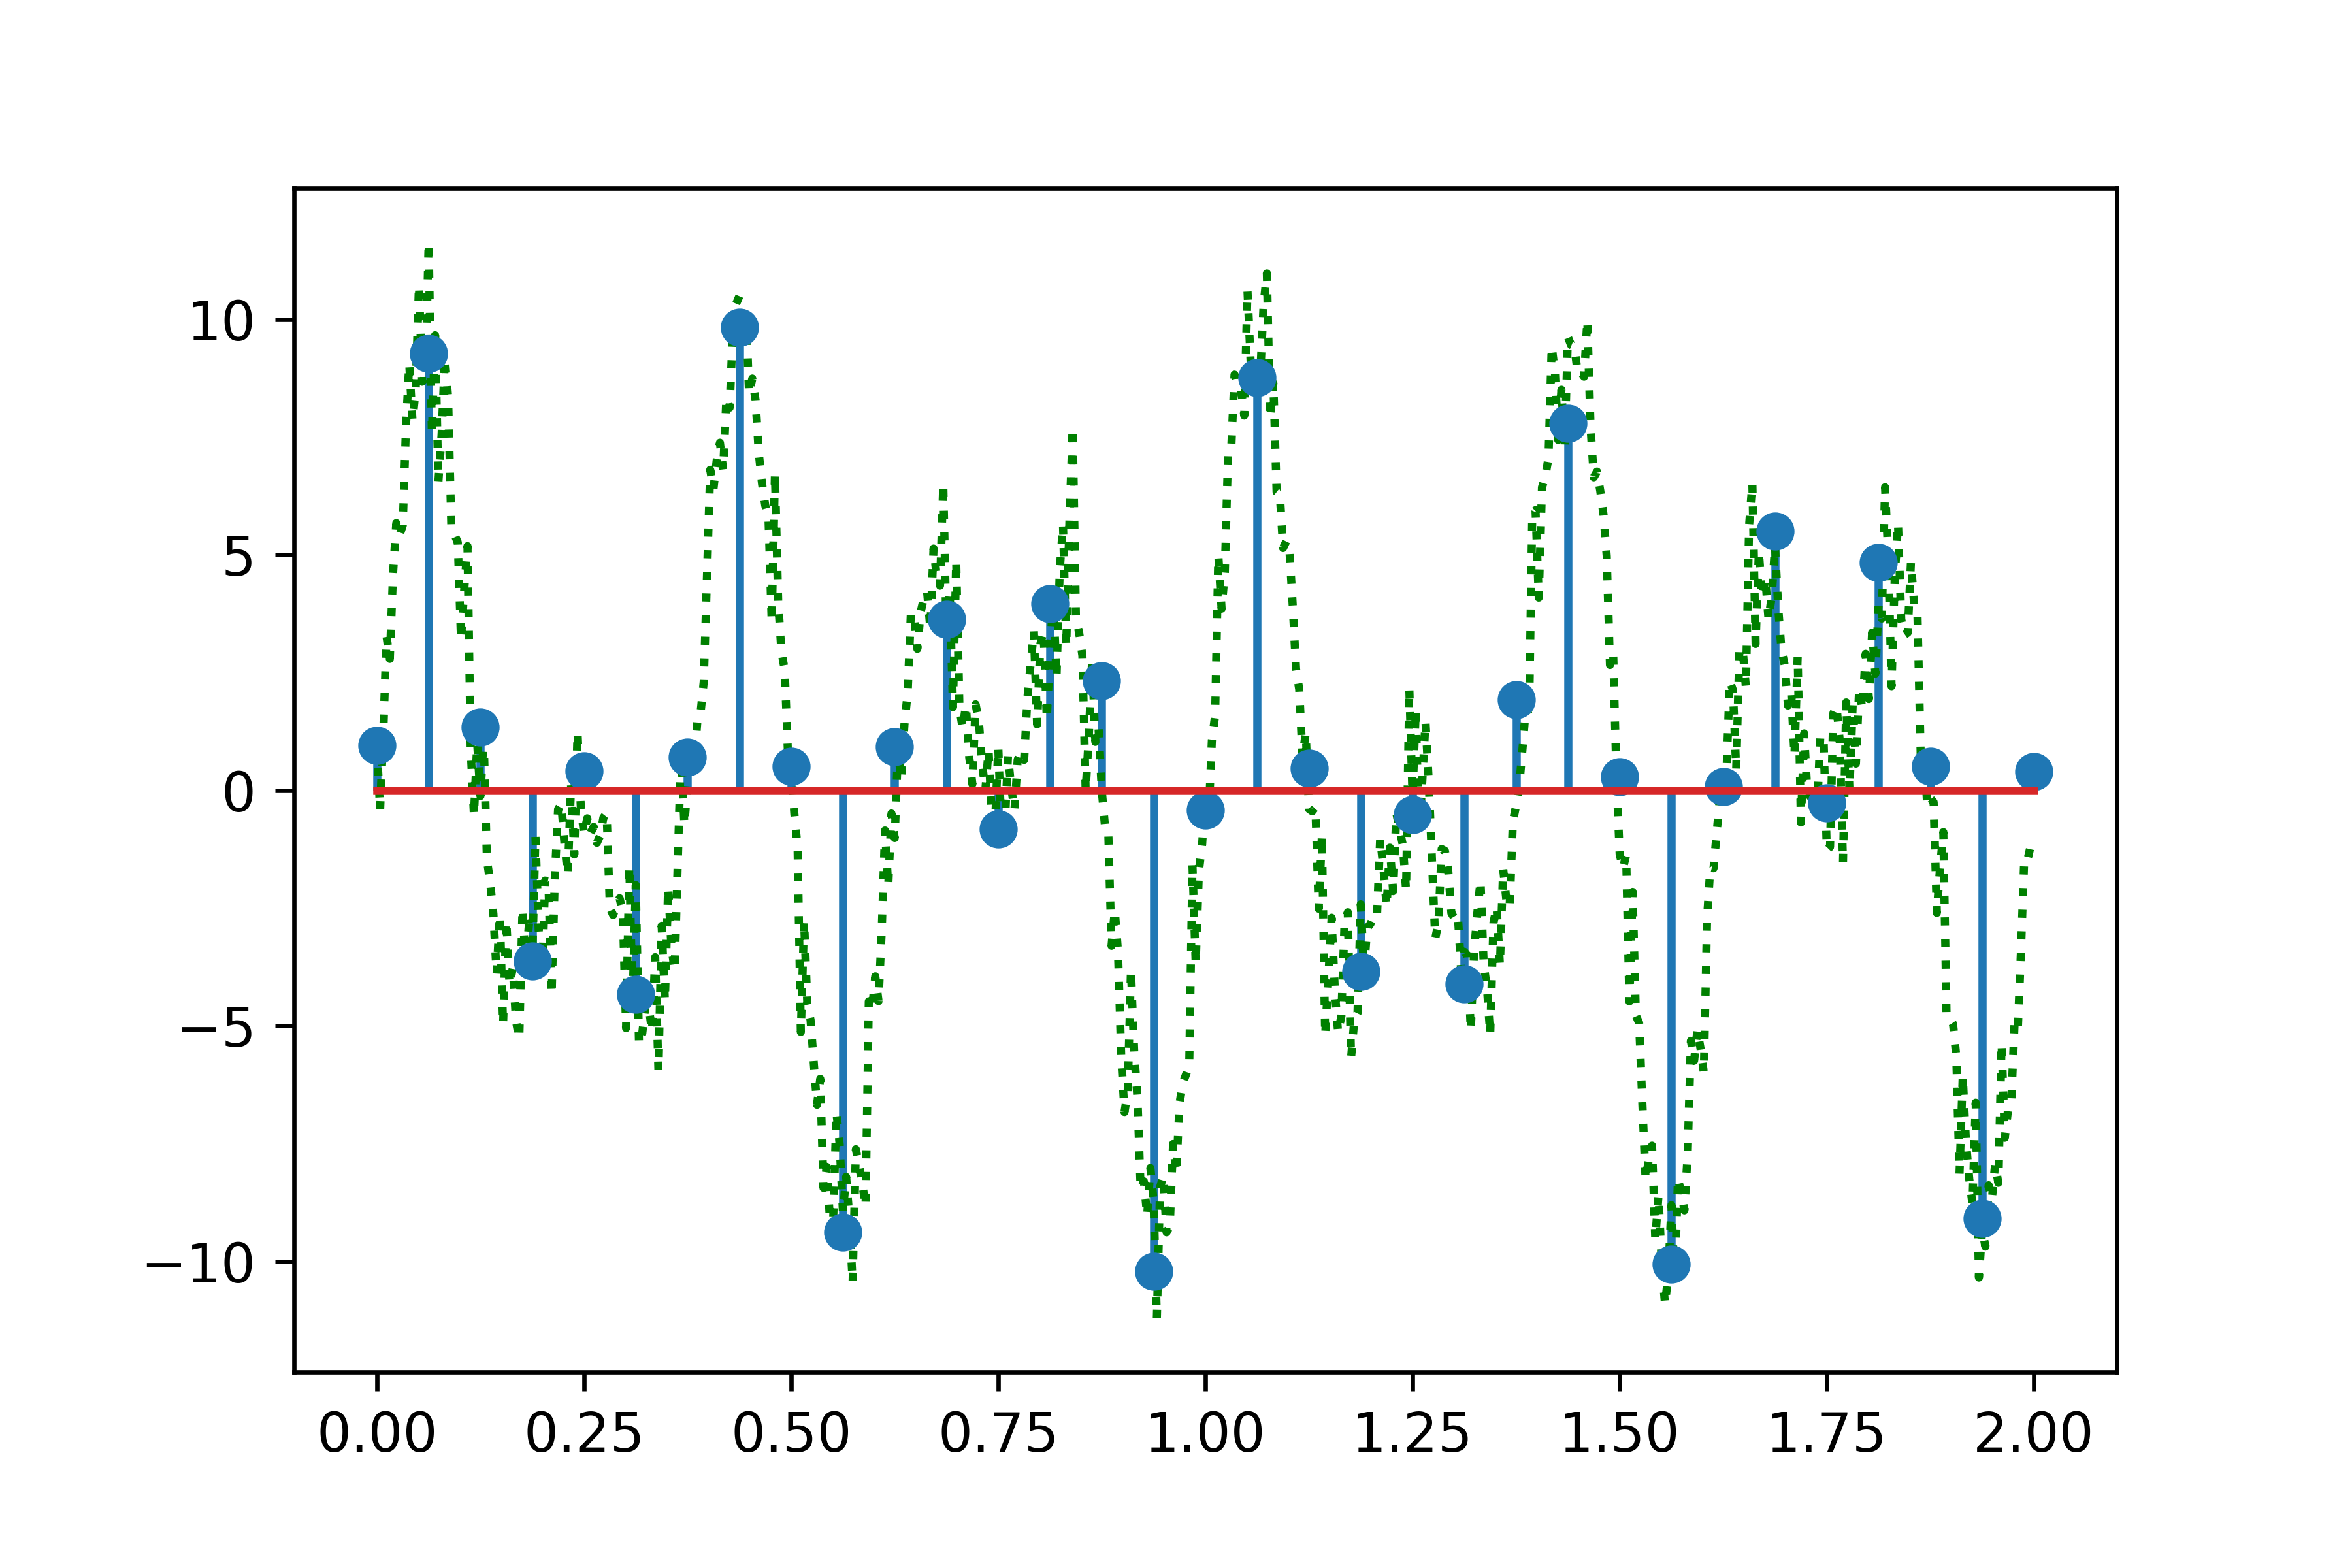
\includegraphics[width=8cm]{sampling.png}
  \caption{謎の信号をサンプリングする}
\end{figure}

\end{block}
\end{frame}

\begin{frame}[fragile]\frametitle{離散Fourier変換}
\begin{exampleblock}{離散Fourier変換(高速Fourier変換ではない!)}
\begin{pygments}{python}
inverse_Fs = [
    sum(
        (1 / sampling_freq)
        * Fs[n]
        * cmath.exp((0 + 2j) 
        * cmath.pi * k * n / sampling_freq)
        for n in range(sampling_freq)
    )
    for k in range(sampling_freq)
]
\end{pygments}
\end{exampleblock}

\end{frame}

\begin{frame}[fragile]\frametitle{離散Fourier変換}
\begin{exampleblock}{信号の周波数スペクトル}
\begin{pygments}{python}
plt.stem(
    range(-sampling_freq // 2, sampling_freq // 2),
    list(map(abs, Fs)),
    use_line_collection=True,
)
\end{pygments}
\end{exampleblock}

\end{frame}

\begin{frame}[fragile]\frametitle{離散Fourier変換}

\begin{block}{例:信号の周波数スペクトル}
\begin{figure}
  \centering
  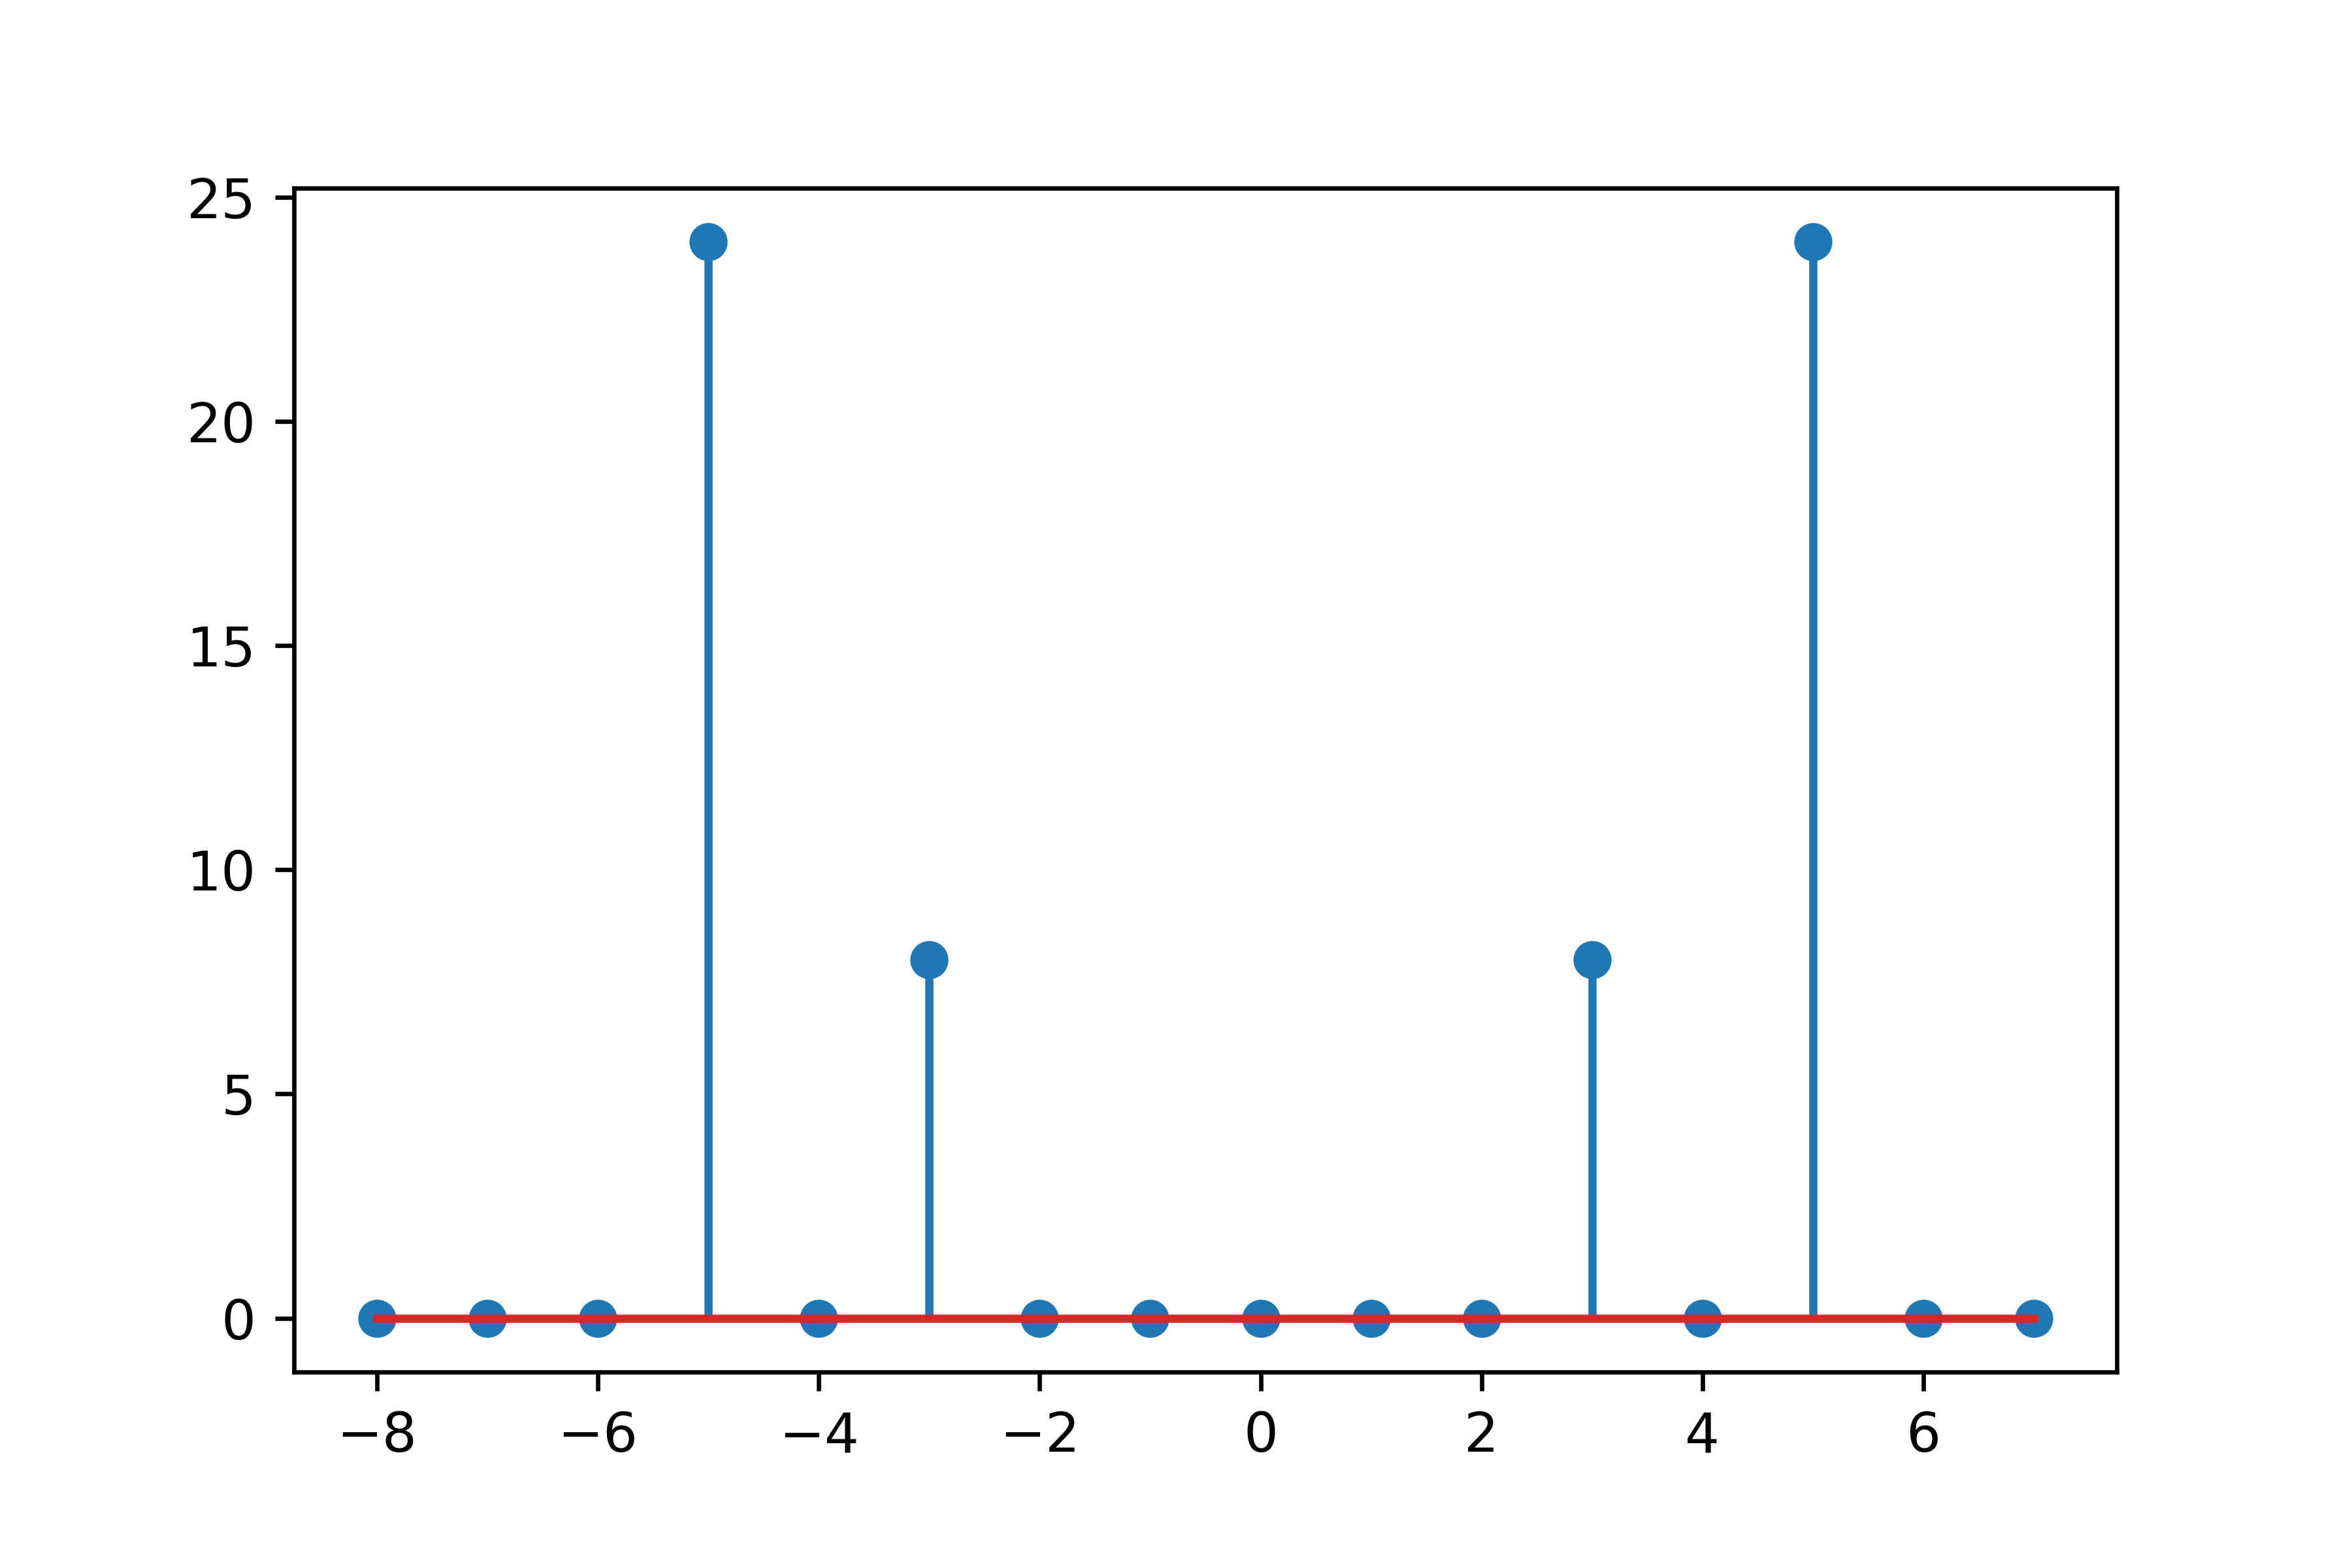
\includegraphics[width=8cm]{stem.png}
  \caption{謎の信号の周波数スペクトル}
\end{figure}

\end{block}
\end{frame}

\section{1の$n$乗根}

\begin{frame}[fragile]\frametitle{1の$n$乗根}

\begin{block}{1の$n$乗根}
1の$n$乗根は
\begin{equation*}
e^{i \frac{2\pi k}{n}}(k=0, \dots , n-1)
\end{equation*}
で与えられる。
\end{block}

\end{frame}

\begin{frame}[fragile]\frametitle{1の$n$乗根}
\begin{exampleblock}{1の$n$乗根で正$n$角形を作図する}
\begin{pygments}{python}
N = 7
roots_of_one = [
    cmath.exp(((2 * cmath.pi * k) / N) * (0 + 1j)) 
    for k in range(N + 1)
]
angles = list(map(cmath.phase, roots_of_one))
length = list(map(abs, roots_of_one))
plt.polar(angles, length)
\end{pygments}
\end{exampleblock}

\end{frame}

\begin{frame}[fragile]\frametitle{1の$n$乗根}

\begin{block}{1の7乗根による正七角形の作図}
\begin{figure}
  \centering
  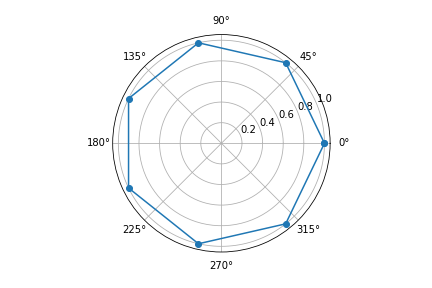
\includegraphics[width=7cm]{heptagon.png}
  \caption{正七角形}
\end{figure}
正七角形は定規とコンパスによって作図ができない。
\end{block}
\end{frame}

\section{まとめ}

\begin{frame}[fragile]\frametitle{まとめ}
\begin{block}{まとめ}
\begin{itemize}
\item \texttt{cmath}は複素数のための数学ライブラリである。
\item 標準ライブラリの範囲でも色々楽しめる。
\item 実運用の場合はNumPyやSciPy、SymPyの活用も検討しましょう。
\end{itemize}
\end{block}
\end{frame}

%%% おまけ %%%
\appendix

\newcounter{finalframe}
\setcounter{finalframe}{\value{framenumber}}

\begin{frame}[fragile]\frametitle{おまけ}
\begin{center}
\Huge{おまけ}
\end{center}
\end{frame}

\section{複素三角函数}

\begin{frame}\frametitle{三角函数}

\begin{block}{余弦函数\texttt{cmath.cos(x)}(公式ドキュメントより)}
$x$の余弦を返します。
\end{block}

\begin{block}{無限級数で定義すればいいんだ!}
\begin{equation*}
\cos{z} := \sum^{\infty}_{n=0}\frac{(-1)^{n}}{(2n)!}z^{2n}.
\end{equation*}
\end{block}

\begin{block}{複素指数函数で定義すればいいんだ!}
\begin{equation*}
\cos{z} := \frac{1}{2}\left(e^{iz} + e^{-iz} \right) 
\end{equation*}
\end{block}

\end{frame}

\begin{frame}[fragile]\frametitle{複素余弦函数を巡る冒険}

\begin{exampleblock}{無限級数による定義}
\begin{pygments}{python}
def cos_by_series(z, n=30):
    return sum(
        (-1) ** i * pow(z, 2 * i) / factorial(2 * i) 
        for i in range(n))
\end{pygments}
\end{exampleblock}

\begin{exampleblock}{複素指数函数による定義}
\begin{pygments}{python}
def cos_by_exp(z):
    i = 0 + 1j
    return (cmath.exp(i * z) + cmath.exp(-i * z)) / 2
\end{pygments}
\end{exampleblock}

\end{frame}

\begin{frame}[fragile]\frametitle{見せてもらおうか、\texttt{cmath.cos}の威力とやらを}
\begin{exampleblock}{自作の関数で$\cos{\pi} = -1$を計算してみる}
\begin{pygments}{python}
>>> z = cmath.pi + 0j
>>> cos_by_series(z)
(-1.0000000000000002+0j)
>>> cos_by_exp(z)
(-1+0j)
\end{pygments}
\end{exampleblock}

\begin{exampleblock}{\texttt{cmath.cos}で$\cos{\pi} = -1$を計算してみる}
\begin{pygments}{python}
>>> cmath.cos(z)
(-1+0j)
\end{pygments}
\end{exampleblock}

\end{frame}


\section{Mandelbrot集合}

\begin{frame}[fragile]\frametitle{Mandelbrot集合}

\begin{block}{Mandelbrot集合}
漸化式
\begin{equation*}
    \left\{
    \begin{alignedat}{4}
          z_{n+1} &= z^{2}_{n} +c \\
          z_{0} &= 0
    \end{alignedat}
    \right.
\end{equation*}
で定義される複素数列$\{z_{n}\}$が発散しないような
複素数$c$全体がなす集合をMandelbrot集合という。
\end{block}

\end{frame}

\begin{frame}[fragile]\frametitle{Mandelbrot集合}

\begin{figure}
  \centering
  
\includegraphics[width=8cm]{mandelbrot.png}
  \caption{Mandelbrot集合(Matplitlibのサンプルコードを改変)}
\end{figure}

\end{frame}

\section{対数螺旋}

\begin{frame}[fragile]\frametitle{対数螺旋}

\begin{block}{対数螺旋}
極座標$(r, \theta)$において$r = ae^{b\theta}$で表される平面曲線を対数螺旋という。
\end{block}

\begin{block}{対数螺旋と複素数}
指数函数は複素数平面上の実数軸にも虚数軸にも平行ではない直線を対数螺旋に写す。
\end{block}

\end{frame}

\begin{frame}[fragile]\frametitle{対数螺旋}

\begin{figure}
  \centering
  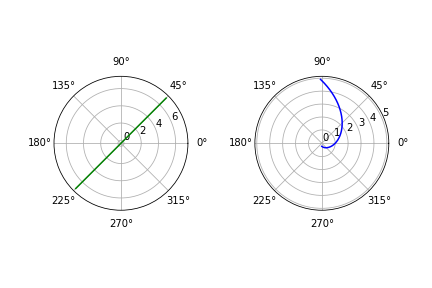
\includegraphics[width=8cm]{log_spiral.png}
  \caption{対数螺旋}
\end{figure}

\end{frame}


\setcounter{framenumber}{\value{finalframe}}
\end{document}
